\documentclass[a4paper, 12pt]{article}%тип документа

%отступы
\usepackage[left=1.5cm,right=1cm,top=2cm,bottom=3cm,bindingoffset=0cm]{geometry}
\setlength{\parindent}{5ex}

%Русский язык
\usepackage[T2A]{fontenc} %кодировка
\usepackage[utf8]{inputenc} %кодировка исходного кода
\usepackage[english,russian]{babel} %локализация и переносы

%Вставка картинок
\usepackage{graphicx}
\graphicspath{{pictures/}}
\DeclareGraphicsExtensions{.pdf,.png,.jpg,}
\usepackage{wrapfig}

%Графики
\usepackage{pgfplots}
\pgfplotsset{compat=1.9}

%Математика
\usepackage{amsmath, amsfonts, amssymb, amsthm, mathtools}

%Таблицы
\usepackage{longtable} 
\usepackage{float}

%Римские цифры
\newcommand{\RomanNumeralCaps}[1]{\uppercase\expandafter{\romannumeral#1}}

\usepackage{multirow}



\begin{document}
	\begin{titlepage}
		\begin{center}
			\textsc{Федеральное государственное автономное образовательное учреждение высшего образования«Московский физико-технический институт (национальный исследовательский университет)»\\[5mm]
			}
			
			\vfill
			
			\textbf{Отчёт по лабораторной работе 5.5.1\\[3mm]
				Измерение коэффициента ослабления потока $ \gamma $-лучей в веществе и определение их энергии
				\\[50mm]
			}
			
		\end{center}
		
		\hfill
		\begin{minipage}{.5\textwidth}
			Выполнил студент:\\[2mm]
			Сериков Василий Романович\\[2mm]
			группа: Б03-102\\[5mm]
			
		\end{minipage}
		\vfill
		\begin{center}
			Москва, 2023 г.
		\end{center}
		
	\end{titlepage}
	
	\newpage
	\setcounter{page}{2}
	\textbf{Аннотация}\\
	
	\textbf{Цель работы: }\\
	
	С помощью сцинтилляционного счетчика измерить линейные коэффициенты ослабления потока $ \gamma $-лучей в свинце, железе и алюминии; по их величине определить энергию $ \gamma $-квантов.\\
	
	\textbf{Теория}\\
	
	Гамма-лучи возникают при переходе возбужденных ядер из одного энергетического состояния в другое, более низкое. Энергия $ \gamma $-квантов обычно заключена между несколькими десятками килоэлектронвольт и несколькими миллионами электрон-вольт. Гамма-кванты не несут электрического заряда, их масса равна нулю. Проходя через вещество, пучок $ \gamma $-квантов постепенно ослабляется. Ослабление происходит по экспоненциальному закону, который может быть записан в двух формах:
	
	\begin{equation}\label{I(mu)}
		I = I_0 e^{-\mu l}, \quad I_o e^{-\mu 'm_1} 
	\end{equation}
	
	В этих формулах $ I, I_0 $ --- интенсивности прошедшего и падающего излучений, $ l $ --- длина пути, пройденного пучком $\gamma$-лучей, $ m_1 $ ---
	масса пройденного вещества, приходящаяся на единицу площади, $ \mu $ и
	$ \mu' $ --- константы, величина которых зависит от вещества, сквозь кото-
	рое проходят $\gamma$-лучи. 
	
	Ослабление потока $\gamma$-лучей, происходящее при прохождении среды, связано с тремя эффектами: фотоэлектрическим поглощением,
	комптоновским рассеянием и с генерацией электрон-позитронных пар.
	
	\textbf{Фотоэлектрическое поглощение.} При столкновении $\gamma$-квантов с
	электронами внутренних атомных оболочек может происходить поглощение квантов. Энергия $\gamma$-кванта передается соответствующему электрону, а импульс делится между этим электроном и оставшимся после
	его вылета ионом. Свободный электрон не может поглотить $\gamma$-квант,
	так как при этом невозможно одновременно удовлетворить законам
	сохранения энергии и импульса. Фотоэффект является доминирующим механизмом поглощения $\gamma$-квантов при не очень высоких энергиях.
	
	\textbf{Комптоновское рассеяние.} Комптоновским рассеянием (или комптоновским эффектом) называется упругое столкновение $\gamma$-кванта с электроном. При таком столкновении $\gamma$-квант передает электрону часть своей энергии, величина которой определяется углом рассеяния. В отличие от фотоэффекта, который может идти только на сильно связанных электронах, комптоновское рассеяние происходит на свободных или слабосвязанных электронах. Роль эффекта Комптона становится
	существенной только тогда, когда энергия квантов становится много
	больше энергии связи электронов в атоме (когда достаточно падает
	вероятность фотоэффекта). Атомные электроны в этом случае можно
	считать практически свободными, что обычно и делается при теоретическом анализе.
	В отличие от фотоэффекта, эффект
	Комптона приводит не к поглощению $\gamma$-квантов, а к их рассеянию и
	уменьшению их энергии.
	
	\textbf{Образование электрон-позитронных пар} При энергиях $\gamma-$лучей выше $2mc^2$ = 1,02 МэВ может происходить их поглощение, связанное с образованием пар. Такое рождение происходит только в электрическом поле ядра. При энергиях больше  $2mc^2$ вероятность образования пар сравнима с вероятностью комптон-эффекта, а фотоэффект уже не играет практически никакой роли.
	
	\textbf{Полный коэффициент ослабления $\gamma$-лучей}
	
	Полный линейный коэффициент $ \mu $ ослабления пучка $\gamma$-квантов при прохождении через вещество равен сумме коэффициентов для всех трех рассмотренных процессов. На рис. \ref{ris mu} изображены графики $ \mu $ для различных материалов.
	
	\begin{figure}[h!]
		\centering
		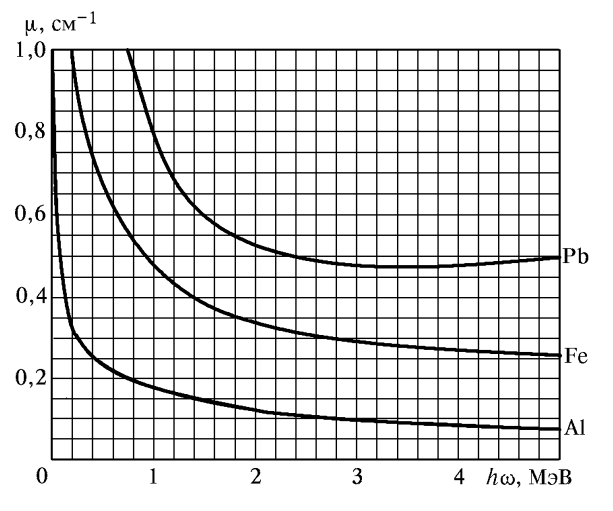
\includegraphics[width=0.6\linewidth]{1}
		\caption{Полные коэффициенты ослабления потока $\gamma$-лучей в алюминии, железе и свинце}
		\label{ris mu}
	\end{figure}
	
	\begin{equation}\label{mu}
		\mu = \dfrac{1}{l} \ln{\dfrac{N_0}{N}}
	\end{equation}
	
	Для определения коэффициента ослабления нужно измерить толщину образца $ l $, число падающих частиц $ N_0 $ и число
	частиц $ N $, прошедших через образец.\\
	
	\textbf{Экспериментальная установка}\\
	
	\begin{figure}[h!]
		\centering
		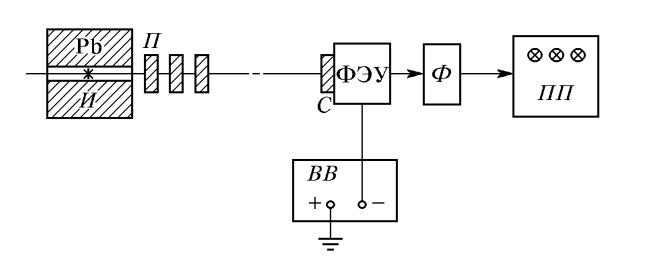
\includegraphics[width=0.7\linewidth]{2}
		\caption{Блок-схема установки, используемой для измерения коэффициентов ослабления потока $\gamma$-лучей: И --- источник $\gamma$-лучей; $ Pb $ --- свинцовый контейнер с коллиматорным каналом; П --- набор поглотителей; С --- сцинтиллятор (кристалл
			NaI(Tl) ); Ф --- формирователь-выпрямитель}
	\end{figure}
	
	Схема установки, используемой в работе, показана на рис.2. Свинцовый коллиматор выделяет узкий почти параллельный пучок $\gamma$-квантов, проходящий через набор поглотителей П и регистрируемый сцинтилляционным счетчиком). Сигналы от счетчика усиливаются и регистрируются пересчетным прибором. Высоковольтный выпрямитель ВВ обеспечивает питание сцинтилляционного счетчика.
	
	При недостаточно хорошей геометрии в результаты опытов могут
	вкрасться существенные погрешности. В реальных установках всегда имеется конечная вероятность того, что $\gamma$-квант провзаимодействует в
	поглотителе несколько раз до того, как попадет в детектор. Чтобы уменьшить число таких случаев, в данной работе сцинтилляционный счетчик расположен на большом расстоянии от источника $\gamma$-квантов, а поглотители имеют небольшие
	размеры.\\
	
	\textbf{Ход работы: }\\
	
	\begin{enumerate}
		
	\item Измерим показания радиационного фона (число n срабатываний счетчика) в течении времени t = 60с, повторив эксперимент 5 раз. Полученные данные занесем в таблицу 1.
			
	\begin{longtable}{|c|c|c|c|c|c|}
		\hline
		№ & 1 & 2 & 3 & 4 & 5\\ \hline
		$n_{\text{фон}}$ & 1521 & 1476 & 1549 & 1604 & 1552 \\ \hline
		\caption{Число срабатываний счетчика при измерении радиационного фона за t = 60 сек}
	\end{longtable}

	Посчитаем среднее значение $\overline{n_{\text{фон}}}$ числа срабатываний счетчика за 15 секунд
	
	$$\overline{n_{\text{фон}}} = \frac{1}{5} \sum_{i = 1}^{5} n_i = 385$$
	
	$$ \sigma_{\overline{n_{\text{фон}}}} = \sqrt{\frac{1}{5(5-1)} \sum_{i = 1}^{5} (\overline{x} - x_i)^2} = 11 $$
	
	\item Измерим число n срабатываний счетчика при полностью открытом коллиматоре, а затем при коллиматоре закрытым свинцовой пробкой в течении 15 секунд, повторив эксперимент 5 раз. Результаты измерений внесем в таблицы 2, 3.
	
	\begin{longtable}{|c|c|c|c|c|c|}
		\hline
		№ & 1 & 2 & 3 & 4 & 5\\ \hline
		$n_{\text{откр}}$ & 119286 & 117668 & 115375 & 114351 & 113526 \\ \hline
		\caption{Число срабатываний счетчика при открытом коллиматоре за t = 15 сек}
	\end{longtable}

	\begin{longtable}{|c|c|c|c|c|c|}
		\hline
		№ & 1 & 2 & 3 & 4 & 5\\ \hline
		$n_{\text{закр}}$ & 331 & 360 & 354 & 367 & 388 \\ \hline
		\caption{Число срабатываний счетчика при закрытом свинцовой пробкой коллиматоре за t = 15 сек}
	\end{longtable}

	Посчитаем среднее значение чисел срабатываний счетчика $\overline{n_{\text{откр}}}$ и $\overline{n_{\text{закр}}}$ по формулам из пункта 1.
			
	$$ \overline{n_{\text{откр}}} = 116041 \pm 3481$$
	$$ \overline{n_{\text{закр}}} = 360 \pm 10$$
				
	\item Исследуем поглощение $\gamma$-лучей в свинце, железе, алюминии, пробке.
	Измерим число частиц, попадающих в счетчик за фиксированное время t = 15 сек. в отсутствие $N_0$ и присутствии $N$ разной толщины L поглотителя. Полученные данные занесем в таблицы 4, 5, 6, 7.
	
	
	\begin{longtable}{|c|c|c|c|c|c|c|c|c|}
		\hline
		№ & 1 & 2 & 3 & 4 & 5 & L, мм &  $\overline{n^{\text{Pb}}}$ & $\varepsilon_{\overline{n^{\text{Pb}}}}$, \% \\ \hline
		$n_{1}^{\text{Pb}}$ & 63341 & 63249 & 62866 & 62804 & 62988 & 4,5 & 63050 & 0,35\\ \hline
		$n_{2}^{\text{Pb}}$ & 35296 & 35328 & 34727 & 34980 & 35192 & 9,5 & 35105 & 0,67\\ \hline
		$n_{3}^{\text{Pb}}$ & 20833 & 21217 & 21028 & 21237 & 20855 & 14 & 21052 & 0,86 \\ \hline
		$n_{4}^{\text{Pb}}$ & 13159 & 12879 & 13223 & 12799 & 12901 & 19 & 12992 & 1,34\\ \hline
		$n_{5}^{\text{Pb}}$ & 7409 & 7414 & 7568 & 7594 & 7323 & 24 & 7462 & 1,44\\
	    \hline
		$n_{6}^{\text{Pb}}$ & 4114 & 4210 & 4182 & 4104 & 4173 & 29 & 4157 & 1,03\\
		\hline
		
		\caption{Число срабатываний счетчика при наличии свинцовых пластин толщины L ($\sigma_L = 0,1$ мм) за t = 15 сек}
	\end{longtable}
	
	
	\begin{longtable}{|c|c|c|c|c|c|c|c|c|}
		\hline
		№ & 1 & 2 & 3 & 4 & 5 & L, мм & $\overline{n^{\text{Fe}}}$& $\varepsilon_{\overline{n^{\text{Fe}}}}$, \% \\ \hline
		$n_{1}^{\text{Fe}}$ & 60490 & 60496 & 60721 & 60765 & 60821 & 10,3 & 60659 & 0,24\\ \hline
		$n_{2}^{\text{Fe}}$ & 34326 & 34083 & 34643 & 34649 & 34601 & 20,5 & 34460 & 0,68 \\ \hline
		$n_{3}^{\text{Fe}}$ & 20032 & 20017 & 20216 & 11920 & 20224 & 30,5 & 20081 & 0,62\\ \hline
		$n_{4}^{\text{Fe}}$ & 11672 & 11747 & 11814 & 11738 & 11826 & 40,6 & 11750 & 1,48\\ \hline
		$n_{5}^{\text{Fe}}$ & 6812 & 6807 & 6865 & 6921 & 6819 & 50,8 & 6844 & 0,65\\ 
		\hline
		$n_{6}^{\text{Fe}}$ & 4089 & 4143 & 4137 & 4322 & 4073 & 61,2 & 4153 & 2,2\\
		\hline
		\caption{Число срабатываний счетчика при наличии железных  пластин толщины L ($\sigma_L = 0,1$ мм) за t = 15 сек}
	\end{longtable}

	\begin{longtable}{|c|c|c|c|c|c|c|c|c|}
		\hline
		№ & 1 & 2 & 3 & 4 & 5 & L, мм & $\overline{n^{\text{Al}}}$ & $\varepsilon_{\overline{n^{\text{Al}}}}$, \%\\ \hline
		$n_{1}^{\text{Al}}$ & 73609 & 73753 & 73311 & 72419 & 72784 & 22 & 73175 & 0,72\\ \hline
		$n_{2}^{\text{Al}}$ & 47980 & 48101 & 48151 & 47688 & 48021 & 40,1 & 47988 & 0,35\\ \hline
		$n_{3}^{\text{Al}}$ & 32223 & 31937 & 33051 & 31711 & 31897 & 60,2 & 32163 & 1,8\\ \hline
		$n_{4}^{\text{Al}}$ & 21359 & 21585 & 21423 & 21572 & 21698 & 80,3 & 21527 & 0,50\\ \hline
		$n_{5}^{\text{Al}}$ & 14755 & 14832 & 14976 & 14733 & 14855 & 
		100,5 & 14830 & 0,60\\ 
		\hline
		\caption{Число срабатываний счетчика при наличии алюминиевых  пластин толщины L ($\sigma_L = 0,1$ мм) за t = 15 сек}
	\end{longtable}

\newpage
	
		\begin{longtable}{|c|c|c|c|c|c|c|c|c|}
		\hline
		№ & 1 & 2 & 3 & 4 & 5 & L, мм & $\overline{n^{\text{Cork}}}$ &  $\varepsilon_{\overline{n^{\text{Cork}}}}$, \%\\ \hline
		$n_{1}^{\text{Cork}}$ & 112080 & 109474 & 109393 & 109608 & 109132 & 24,7 & 109937 & 1,04\\ \hline
		$n_{2}^{\text{Cork}}$ & 105602 & 106388 & 105002 & 106197 & 105960 & 44,4 & 105829 & 0,48\\ \hline
		$n_{3}^{\text{Cork}}$ & 103133 & 103245 & 102893 & 103591 & 102547 & 64,4 & 103081 & 0,35\\ \hline
		$n_{4}^{\text{Cork}}$ & 100900 & 101702 & 102039 & 101557 & 101004 & 82,7 & 101440 & 0,44\\ \hline
		\caption{Число срабатываний счетчика при наличии пробковых  пластин толщины L ($\sigma_L = 0,1$ мм) за t = 15 сек}
	\end{longtable}

	
	\item По полученным данным построим графики зависимости логарифма числа зафиксированных частиц от толщины пластин с учетом фонового числа частиц.
	
 	\begin{figure}[h]
		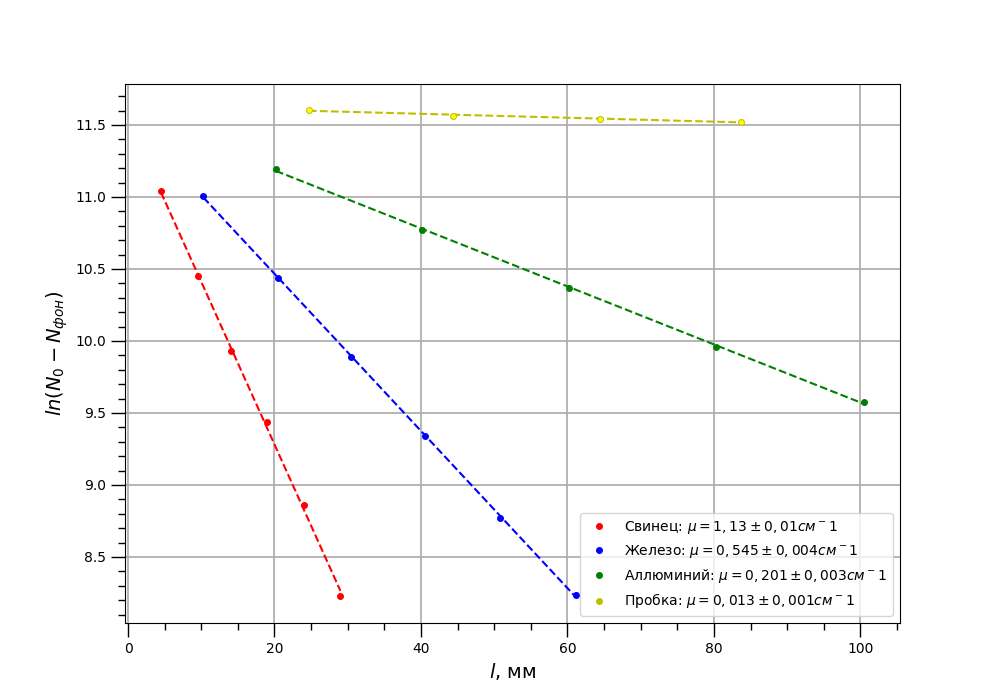
\includegraphics[scale=0.7]{graph.png}
		\centering
		\caption{График зависимости логарифма числа зафиксированных частиц от толщины пластин}
	\end{figure}
	
	Погрешность вычисления коэффициента поглощения в точке задается следующей формулой: 
	
	$$ \sigma_{\mu} = \sqrt{ \left(\frac{\sigma_{N-N_0}}{l(N-N_0)} \right)^2 + \left(\frac{\sigma_{N-N_0} \ln(N-N_0)}{l^2}\right)^2} $$
	
	Погрешность МНК задаются формулой:
	
	$$ \sigma_{\mu}^{\text{МНК}} = \frac{1}{\sqrt{i}} \sqrt{\frac{<\ln(N-N_0)^2> - <\ln(N-N_0)>^2}{<l^2> - <l>^2} - \mu^2} $$
	
	Тогда полная погрешность коэффициента поглощения:
	
	$$ \sigma_{\Sigma} = \sqrt{\overline{\sigma_{\mu}}^2 + {(\sigma_{\mu}^{\text{МНК}})}^2 } $$
	
	
\item 	По таблице соответствия коэффициентов поглощения энергиям определим среднюю энергию $\gamma$-лучей, испускаемых источником.\\
	
	1) 1,13$\pm 0,01\text{ см}^-1$ -> 0,7МэВ - для свинца\\
	2) 0,545$\pm 0,004\text{ см}^-1$ -> 0,7МэВ - для железа\\
	3) 0,201$\pm 0,003\text{ см}^-1$ -> 0,7МэВ - для алюминия\\
	
	\item Рассчитаем коэффициенты $\mu'$ по формуле:
	
	$$ \mu' = \mu/\rho, \text{		где $\rho$ - плотность материала пластин}$$ 
	
	Все полученные значения занесем в таблицу 8
	
	\begin{longtable}{|c|c|c|}
		\hline
		&    $\mu$, см$^{-1}$  & $\mu'$, см$^2$/г  \\ \hline
		Pb & $1,13\pm0,01$     & $0,098\pm0,001$   \\ \hline
		Fe & $0,545\pm0,004$    & $0,068\pm0,001$   \\ \hline
		Al & $0,201\pm0,003$    & $0,074\pm0,001$   \\ \hline
		Cork& $0,0136\pm0,0004$    & $0,029\pm0,001$   \\ \hline
		
		\caption{Итоговые данные для коэффициентов ослабления}
	\end{longtable}
	
	
	
	\end{enumerate}
	
	
	
	\textbf{Обсуждение результатов и выводы: }\\
	
	В ходе данной работы мы исследовали ослабление потока $\gamma$-квантов в различных веществах. Определили коэффициенты поглощения для каждого материала. По табличным данным и результатам эксперимента определили энергию $\gamma$-квантов (0,7 МэВ).
	
	Полученные результаты согласуются с табличными данными в пределах погрешности. Вклад в ошибку дают погрешности среднего значения числа зарегистрированных частиц и погрешность измерения длины пластин. Ошибку можно уменьшить, если набирать большее количество данных. 
	
	
	
	
	
	
	
	
	
	
	
	
	
	
	
	
	
	\end{document}